\documentclass[tikz,border=4pt]{standalone}
\usepackage{pgfplots}
\pgfplotsset{compat=1.18}

\begin{document}
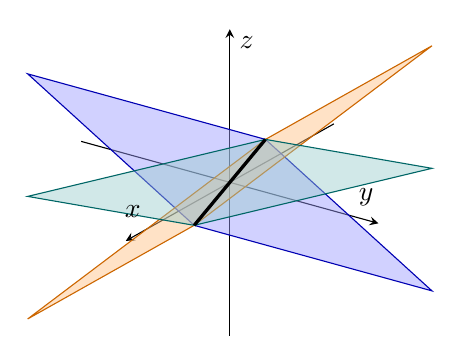
\begin{tikzpicture}
\begin{axis}[
    view={125}{25},
    axis lines=center,
    xlabel={$x$},
    ylabel={$y$},
    zlabel={$z$},
    xmin=-2.5, xmax=2.5,
    ymin=-2.5, ymax=2.5,
    zmin=-2.5, zmax=2.5,
    xtick=\empty, ytick=\empty, ztick=\empty,
    width=8cm, height=8cm,
    clip=false
]

% Plane 1: z = x (blue)
\addplot3[
    surf,
    shader=flat,
    draw=blue!70!black,
    fill=blue!40,
    fill opacity=0.45,
    samples=2,
    domain=-2:2,
    y domain=-2:2
] {x};

% Plane 2: z = y (orange)
\addplot3[
    surf,
    shader=flat,
    draw=orange!80!black,
    fill=orange!50,
    fill opacity=0.45,
    samples=2,
    domain=-2:2,
    y domain=-2:2
] {y};

% Plane 3: z = 0.5x + 0.5y (teal)
\addplot3[
    surf,
    shader=flat,
    draw=teal!80!black,
    fill=teal!40,
    fill opacity=0.45,
    samples=2,
    domain=-2:2,
    y domain=-2:2
] {0.5*x + 0.5*y};

% Line of intersection: (t, t, t)
\addplot3[
    domain=-2:2,
    samples=2,
    very thick,
    black
] ({x}, {x}, {x});

\end{axis}
\end{tikzpicture}
\end{document}
